\section{Results}\label{sec:results}

This section presents the results obtained from running the experiments described in Section \ref{sec:experumnent_executuon}. The Android Runner code, Python scripts for the execution, raw data, and R scripts of the data analysis are publicly available on:
\url{https://github.com/TheEnergyEngineers/ClutteredJS}. Before the results are presented, we want to note that during the execution, the smartphone was unable to load \url{typeform.com} from the `Large' size category, and \url{rt.com} from the `Small' size category. To re-balance the data we randomly selected and removed  \url{ae.godaddy.com} from the `Medium' size category. This resulted in 9 subjects per category resulting in 3 (blocks) $x$ (9 (cluttered mobile web apps) $+$ 9 (de-cluttered mobile web apps)) $x$ 15 (trial repetitions) $=$ 810 measurements.


\subsection{Intrinsic Variability}

\begin{figure}[h]
\centering
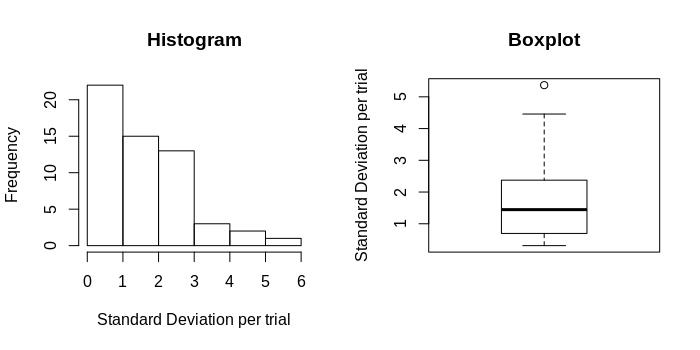
\includegraphics[width=9cm]{reportTemplate/figures/variance.png}
\caption{Variance in the repeated trials} \label{fig:trial_variance}
\end{figure}

We aggregated the raw data by calculating the average energy consumption and standard deviation over the 15 repetitions of each trial. In the remaining graphs and results, we use the average energy consumption for each (cluttered and de-cluttered) subject over these 15 repetitions. First, we discuss the standard deviations (SDs) of the trials to understand if the data is influenced by external factors. Ideally, the SD for each trial should be low as each experiment run with the same subject and cluttering state should have a similar energy consumption in a non-corrupted experiment setting. 

\newpage

The variability of the trials is visualized in Figure \ref{fig:trial_variance}. In the histogram, we observe that most trials have an SD between 0 and 1. The second\-largest groups have an SD between 1 and 3. The remaining subjects have an SD between 4 and 6. From the box plot, we observe that most subjects have indeed small SDs. However, there are some outliers and subjects with a larger SD.

\subsection{Data Distribution}

\begin{figure}[h]
\centering
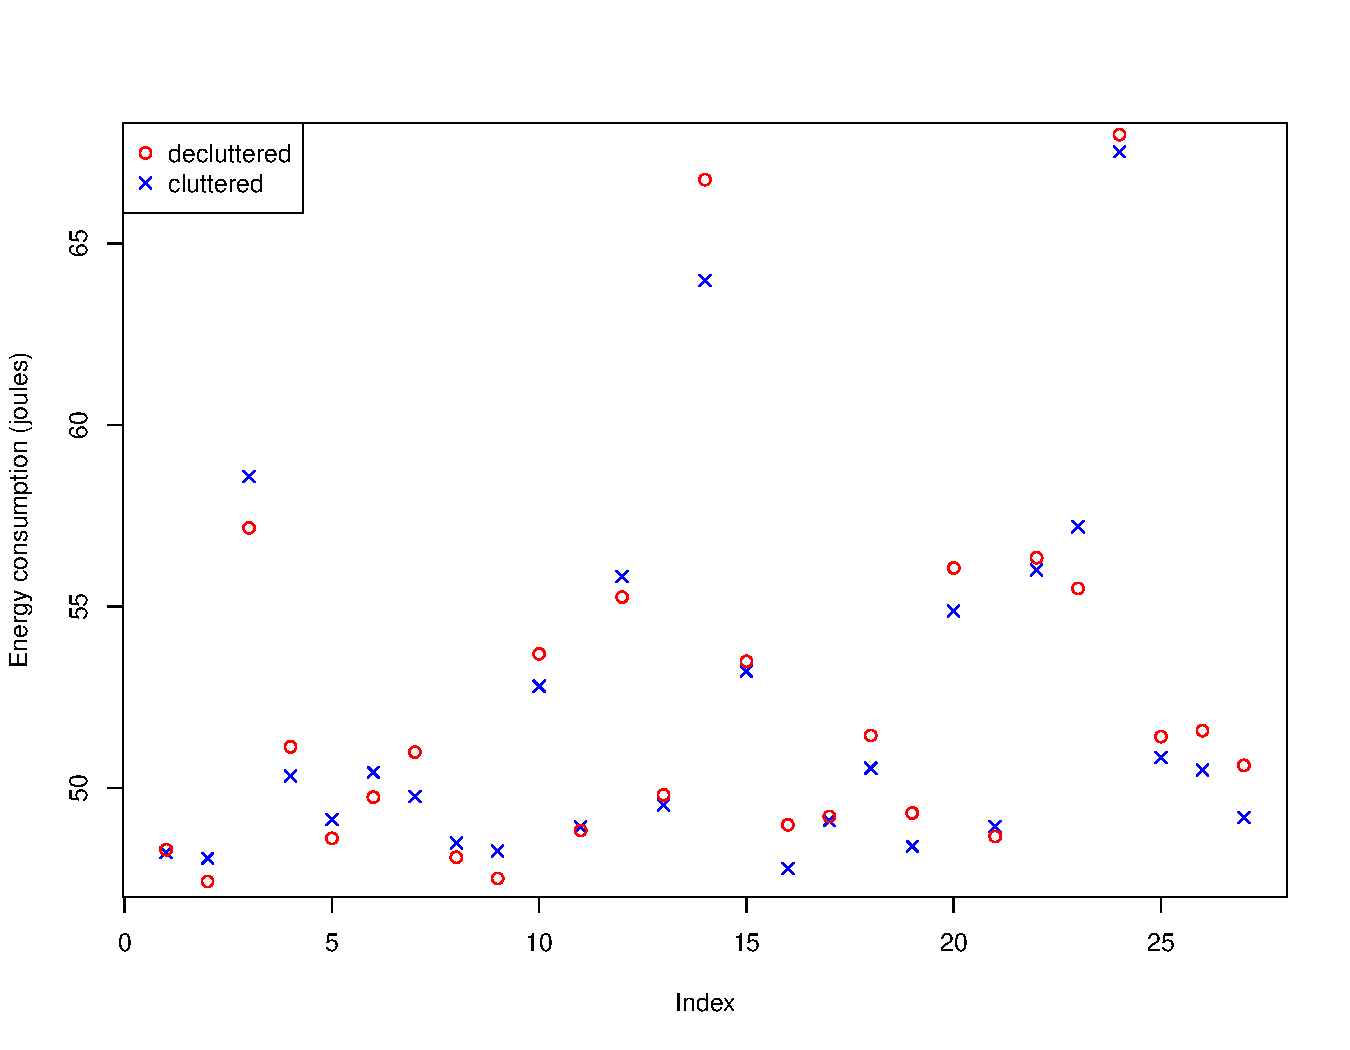
\includegraphics[width=9cm]{reportTemplate/figures/data_distribution/pl1.pdf}
\caption{Cluttered and de-cluttered joule measurements} \label{fig:clutter-declutter-data-all}
\end{figure}

Second, we present the data distributions of the average (over the 15 repetitions) energy consumption for each cluttered and de-cluttered mobile web app. Figure \ref{fig:clutter-declutter-data-all} presents a scatter plot containing the energy measurement for all subjects. From this figure, we observe that the measurements of the de-cluttered mobile web apps are close to the measurements of the cluttered mobile web apps.

\begin{figure}[h]
\centering
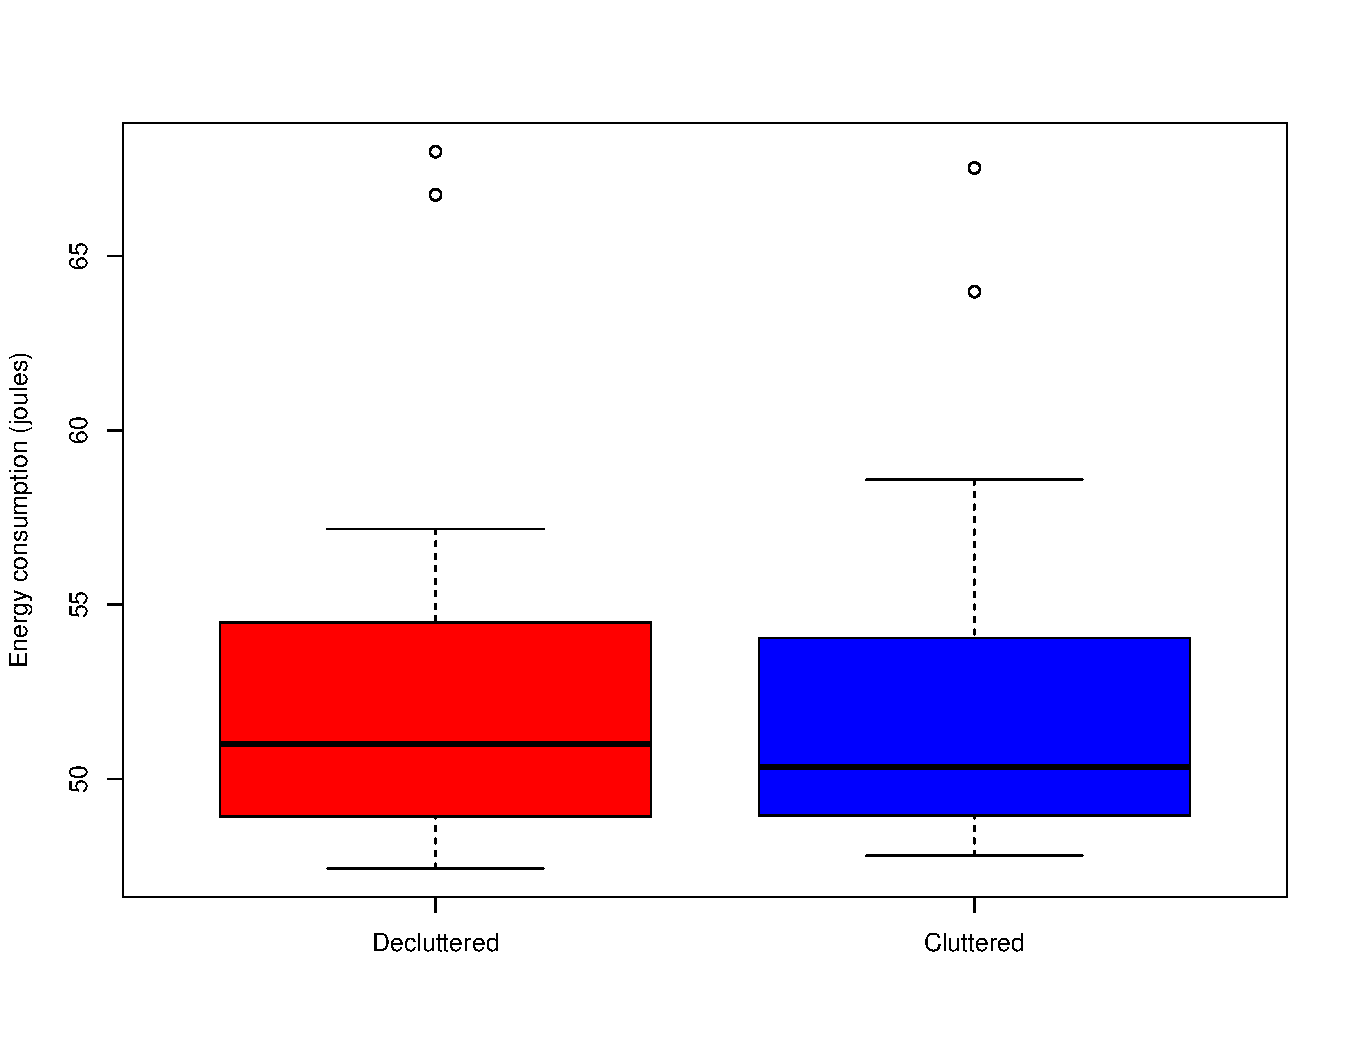
\includegraphics[width=9cm]{reportTemplate/figures/data_distribution/pl2.pdf}
\caption{Boxplot of the energy consumption for cluttered and de-cluttered mobile web apps} \label{fig:boxplot-clutter-vs-declutter}
\end{figure}

\begin{figure}[h]
\centering
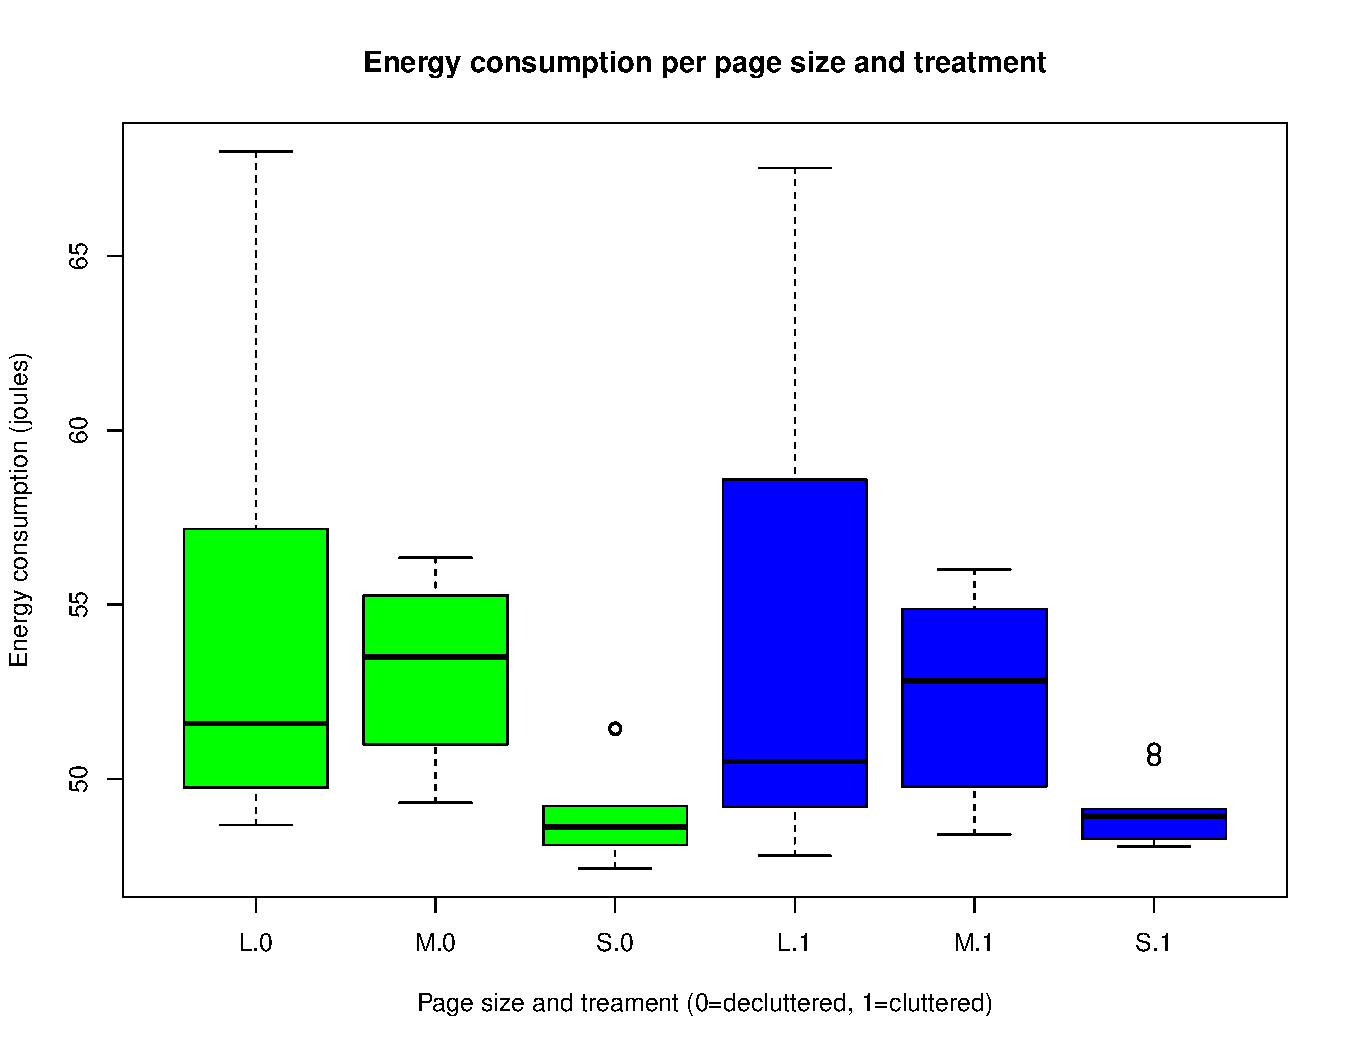
\includegraphics[width=9cm]{reportTemplate/figures/data_distribution/pl3.pdf}
\caption{Boxplot of the energy consumption for cluttered and de-cluttered mobile web apps, blocked into three page size classes} \label{fig:boxplot-clutter-vs-declutter-3-size-classes}
\end{figure}

\newpage
Next, from the box plot in Figure \ref{fig:boxplot-clutter-vs-declutter} we observe that the mean energy consumption of the cluttered treatment is lower than the mean energy consumption of the de-cluttered treatment. This gives an indication that the de-cluttered mobile web apps do not have a smaller energy consumption, without taking into account the page size. To further visually analyze the difference between the two treatments, we take into account the page size and visualize this in Figure \ref{fig:boxplot-clutter-vs-declutter-3-size-classes}. We observe that the smallest page size has indeed the smallest mean energy consumption for both treatments. This is expected as a small mobile web app takes fewer system resources to load compared to larger mobile web apps. However, medium-sized mobile web pages break this pattern as, for both treatments, we observe that the medium page size has a higher mean energy consumption compared to the pages in the `Large' category. 

\subsection{Testing Normality}

\begin{figure}[h]
\centering
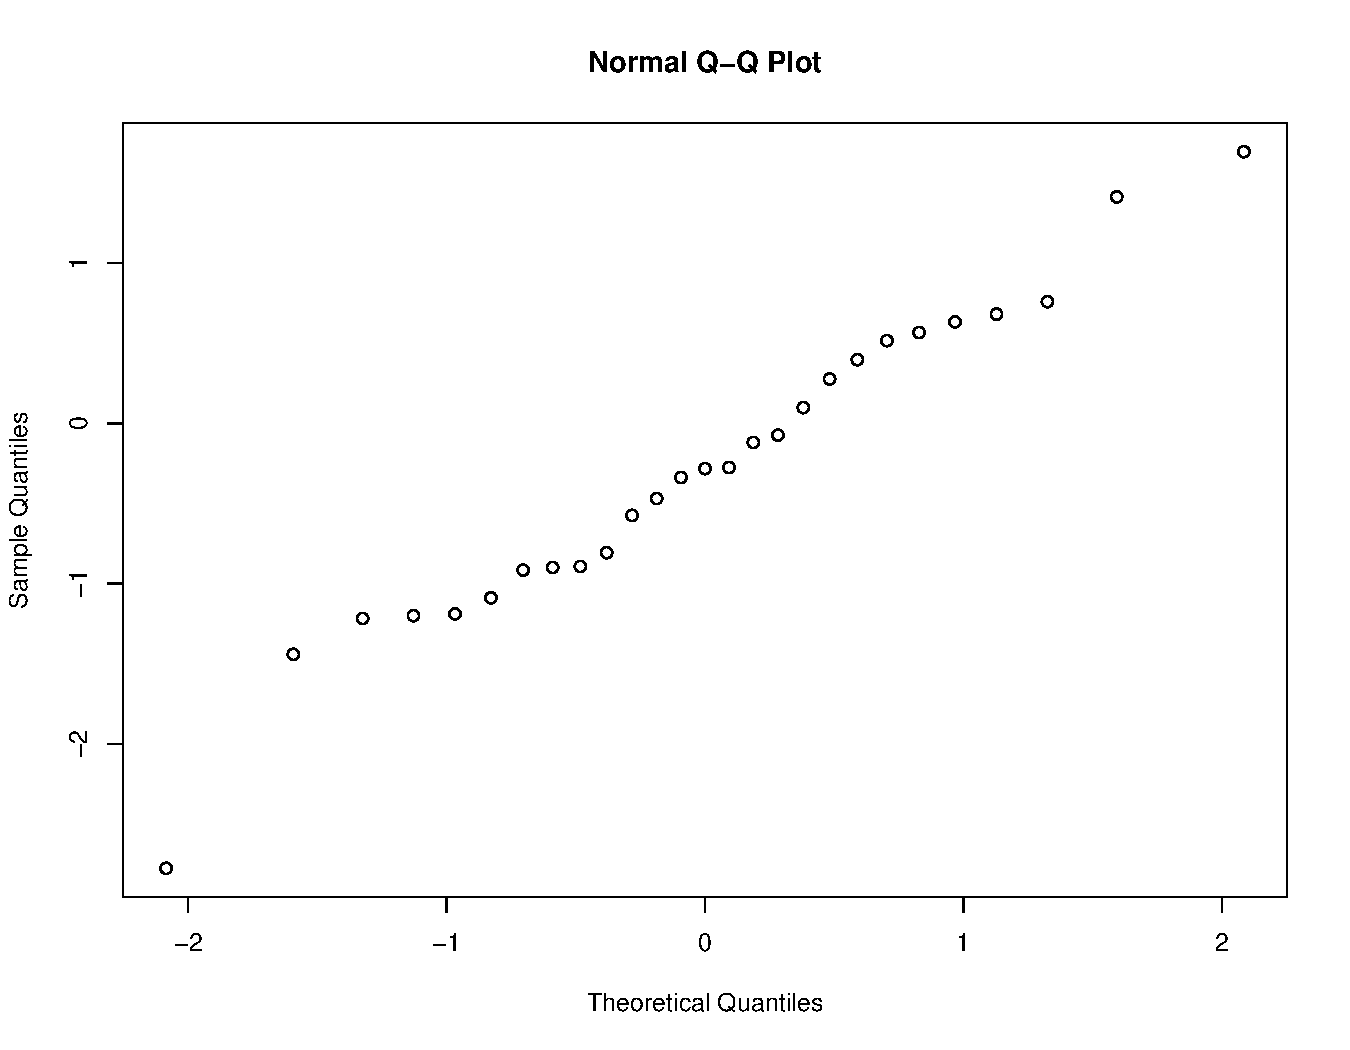
\includegraphics[width=9cm]{reportTemplate/figures/data_distribution/pl4.pdf}
\caption{Q-Q Plot of the difference between the cluttered and de-cluttered results} \label{fig:qq-plot-difference}
\end{figure}

Following the visualizations we test whether the data is normally distributed to determine which test is appropriate. In addition, we check if the difference between the treatments is normally distributed. This is required as a paired t-test is only applicable to data coming from a normal distribution. To execute these normality tests, we used the Shapiro-Wilk normality test. From this, we found a p-value of $0.746$, from which we conclude that the data is normally distributed. However, because the sample is quite small (27) and the Shapiro-Wilk test has a limited accuracy on a small sample size, we also perform a visual inspection using a Q-Q Plot. This plot is shown in Figure~\ref{fig:qq-plot-difference}. From this plot, we observe that the data is indeed approximately normally distributed as the data follows the diagonal line. This allows us to perform the paired t-tests.

\subsection{Paired t-tests}

Finally, we evaluated our hypothesis by executing paired t-tests on the observed data. First, we test whether the cluttered treatment has a significantly different mean compared to the de-cluttered treatment, without taking the page size into account. This test result is a p-value of $0.1472$. Using the significance level $\alpha$ of $0.05$ we conclude that without taking the page size into account, there is no significant difference in the energy consumption between the two treatments. Next, to test whether the treatment matters for the different page sizes, we run a paired t-test for each page individual page size category. From this, we find the following p-values: $0.6699$, $0.01402$, and $0.5268$ for the small, medium, and large page size categories respectively. Using the p threshold of $\frac{0.05}{3} = 0.016$, which is determined by the Bonferroni correction, we conclude that all three are insignificant. As the results are insignificant the effect size is irrelevant.